\documentclass[tikz,border=2pt]{standalone}
\usepackage{amsmath,amssymb}
\usetikzlibrary{arrows.meta}
\begin{document}
% Cycles alternate: length 1 with reward 1, length 3 with reward 9 (reward earned linearly).
% Epochs T = 0,1,4,5,8; R(T_k) = 0,1,10,11,20. alpha = 1/2, Z = 5, R = alpha Z = 2.5:
% the line of slope 2.5 through the origin meets R(t) at t = 4 and t = 8.
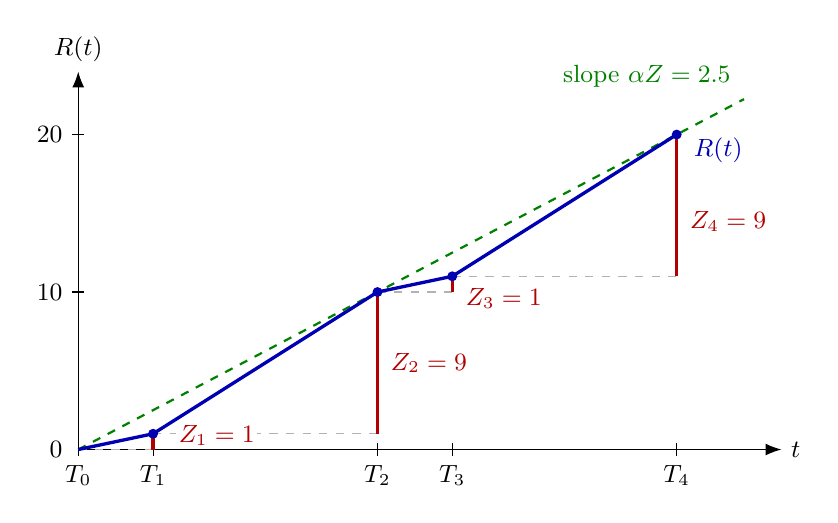
\begin{tikzpicture}[font=\small, >={Latex[length=2mm]}, x=0.95cm, y=0.2cm]
  % axes
  \draw[->] (0,0) -- (9.4,0) node[right] {$t$};
  \draw[->] (0,0) -- (0,24) node[above] {$R(t)$};
  \foreach \y in {10,20} {\draw (0.08,\y) -- (-0.08,\y) node[left] {$\y$};}
  \node[left] at (-0.08,0) {$0$};
  \foreach \x/\k in {0/0,1/1,4/2,5/3,8/4}
    {\draw (\x,0.4) -- (\x,-0.4) node[below] {$T_{\k}$};}
  % helper lines: previous level carried to the next epoch
  \foreach \a/\b/\y in {0/1/0, 1/4/1, 4/5/10, 5/8/11}
    {\draw[gray!60, thin, dashed] (\a,\y) -- (\b,\y);}
  % long-run rate
  \draw[green!50!black, thick, dashed] (0,0) -- (8.9,22.25);
  \node[green!50!black, anchor=south east] at (8.85,22.4) {slope $\alpha Z=2.5$};
  % cumulative reward
  \draw[blue!70!black, very thick] (0,0) -- (1,1) -- (4,10) -- (5,11) -- (8,20);
  \node[blue!70!black, anchor=west] at (8.1,19) {$R(t)$};
  % cycle rewards
  \foreach \x/\a/\b/\k/\z in {1/0/1/1/1, 4/1/10/2/9, 5/10/11/3/1, 8/11/20/4/9}
    {\draw[red!70!black, very thick] (\x,\a) -- (\x,\b);}
  \node[red!70!black, anchor=west, fill=white, inner sep=1pt] at (1.3,0.9) {$Z_1=1$};
  \node[red!70!black, anchor=west] at (4.05,5.5) {$Z_2=9$};
  \node[red!70!black, anchor=west] at (5.05,9.6) {$Z_3=1$};
  \node[red!70!black, anchor=west] at (8.05,14.5) {$Z_4=9$};
  \foreach \x/\y in {1/1, 4/10, 5/11, 8/20} {\fill[blue!70!black] (\x,\y) circle (1.8pt);}
\end{tikzpicture}
\end{document}
